
% \vspace{- 1.5 cm}
\subsubsection{Decision Trees}
For finding the optimal Decision tree, we looked at $11 \times 2 = 22$ different models: 10 different pruning levels (+ no pruning at all) and 2 different impurity measures: Entropy (or \texttt{deviance}) and Gini (or \texttt{gdi}) (\cite[eq. 8.2-8.3]{coursenotes}). In all cases, a full tree is grown i.e. without early stopping before pruning. (One could also have chosen to include early stopping as a parameter to optimize in the cross-validation algorithm. However, in theory at least, it should always be as good or better to prune a fully grown tree rather than stopping the growth early, which is why we chose to omit that parameter from the analysis).  
% \vspace{- 0.2 cm}

\begin{figure}[H]
    \centering
    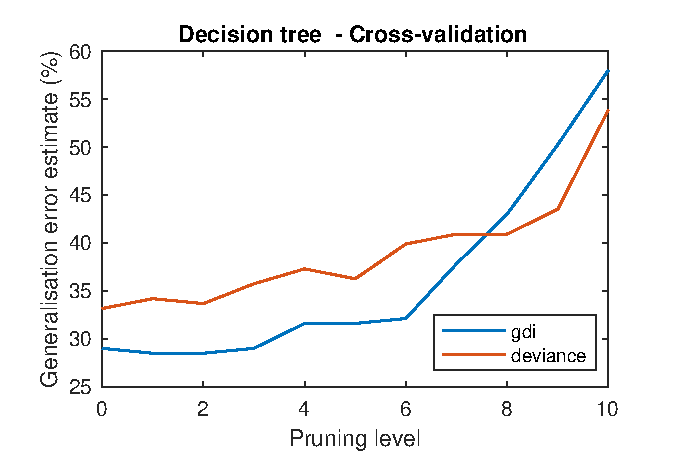
\includegraphics[width = 0.45\textwidth]{fig/dt-crossval.eps}
    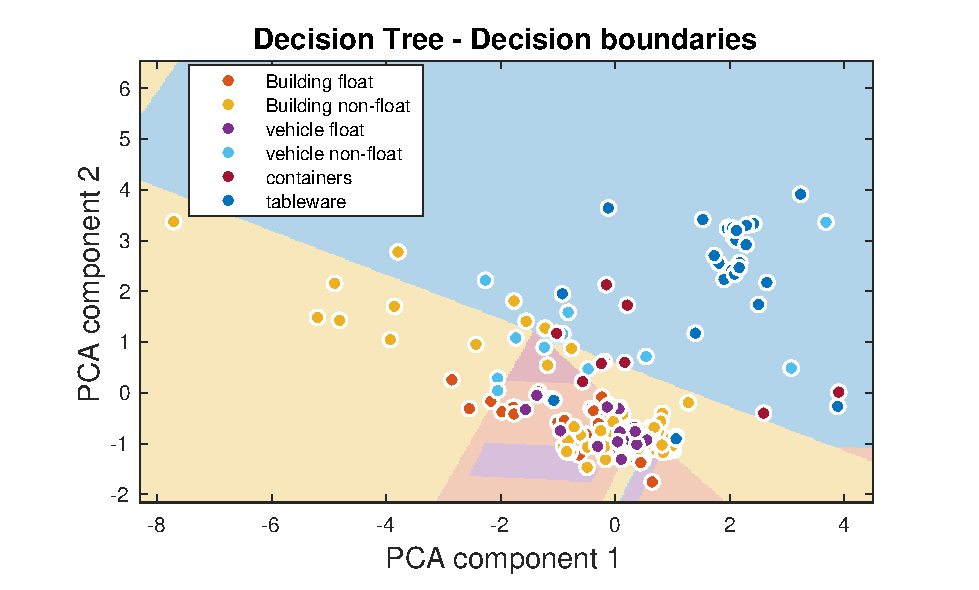
\includegraphics[width=0.5\textwidth]{fig/dt-decision-bounds.eps}
    \caption{\textbf{Left}: Generalization error estimates decision trees as a function of pruning level for two different impurity measures. The models are fitted to the training sets of the inner CV loop, and the generalization error estimates is the average of the error rates when these models are applied to the validation sets in the inner CV loops. \textbf{Right}:Decision bounds of the best decision tree model fitted to the training set of the outer CV loop. The data points are also from the training set.}
    \label{dt-plots}
\end{figure}


From the generalization error estimates shown in Figure \ref{dt-plots}, we find that the Gini impurity measure is the best one with a pruning level P = 1 (one could also have chosen P = 2). This model trained on the whole data set is illustrated appendix \ref{dt-illustration}, and its decision boundaries projected down on the two first principal components are shown in Figure \ref{dt-plots}. Finally, an estimate of its generalization error is found by computing the classification error rate on the test set in the outer CV loop, which is shown in table \ref{classification-performance}.

% \begin{figure}[H]
%     \centering
%     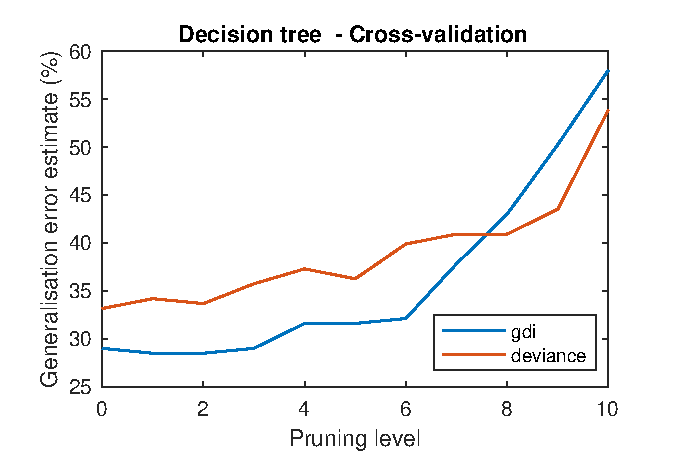
\includegraphics[width = 0.8\textwidth]{fig/dt-crossval.eps}
%     \caption{Generalization error estimates decision trees as a function of pruning level for two different impurity measures. The models are fitted to the training sets of the inner CV loop, and the generalization error estimates is the average of the error rates when these models are applied to the validation sets in the inner CV loops.}
%     \label{dt-crossval}
% \end{figure}

% \begin{figure}[H]
%     \centering
%     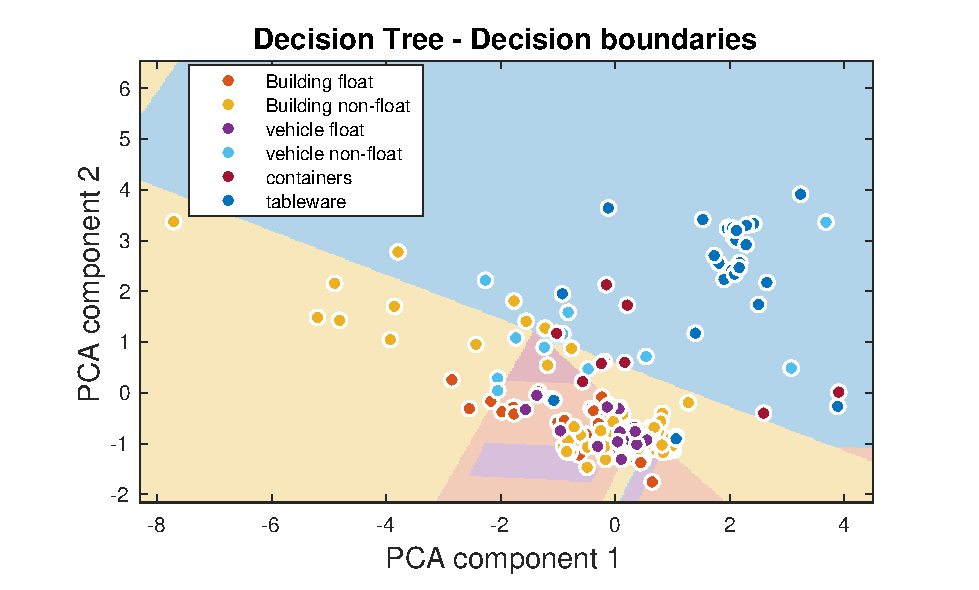
\includegraphics[width = 0.6\textwidth]{fig/dt-decision-bounds.eps}
%     \caption{Decision bounds of the decision tree projected down on the two first principal components.}
%     \label{dt-decision-bounds}
% \end{figure}

% \begin{figure}[h]
 
% \begin{subfigure}{0.5\textwidth}
% 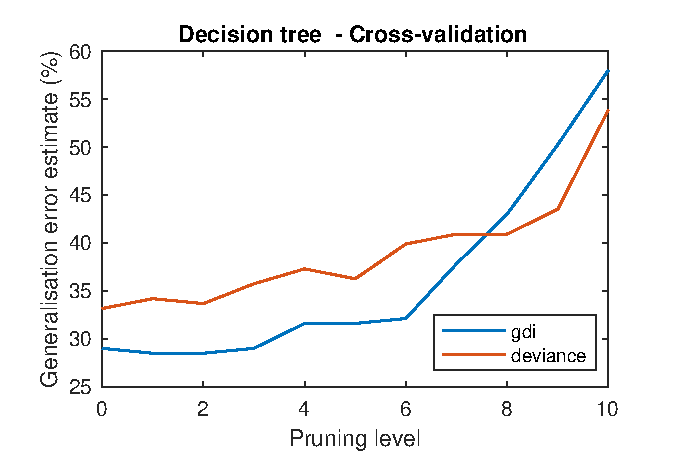
\includegraphics[width = 0.5\textwidth]{fig/dt-crossval.eps} 
% \caption{Caption1}
% \label{fig:subim1}
% \end{subfigure}
% \begin{subfigure}{0.5\textwidth}
% 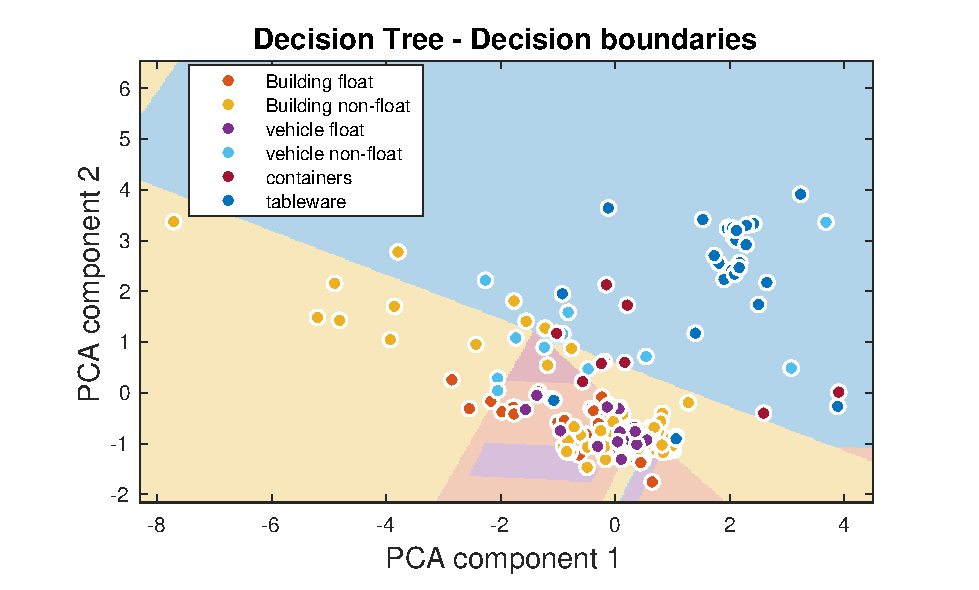
\includegraphics[width=0.9\linewidth, height=5cm]{fig/dt-decision-bounds.eps}
% \caption{Caption 2}
% \label{fig:subim2}
% \end{subfigure}
 
% \caption{Caption for this figure with two images}
% \label{fig:image2}
% \end{figure}

